% author:   sam tenka
% change:   2022-05-23
% create:   2022-05-11

%==============================================================================
%=====  0.  DOCUMENT SETTINGS  ================================================
%==============================================================================

%~~~~~~~~~~~~~~~~~~~~~~~~~~~~~~~~~~~~~~~~~~~~~~~~~~~~~~~~~~~~~~~~~~~~~~~~~~~~~~
%~~~~~~~~~~~~~  0.0. About this Exposition  ~~~~~~~~~~~~~~~~~~~~~~~~~~~~~~~~~~~

%---------------------  0.0.0. page geometry  ---------------------------------
\documentclass[11pt, justified]{tufte-book}
\geometry{
  left           = 0.90in, % left margin
  textwidth      = 4.95in, % main text block
  marginparsep   = 0.15in, % gutter between main text block and margin notes
  marginparwidth = 2.30in, % width of margin notes
                 % 0.20in  % width from margin to edge
}

%---------------------  0.0.1. math packages  ---------------------------------
\newcommand\hmmax{0}
\newcommand\bmmax{0}
\usepackage{amsmath, amssymb, amsthm, mathtools, bm, euler}
\usepackage{listings}
\usepackage{xstring}%hanging, txfonts, ifthen}

%---------------------  0.0.2. graphics packages  -----------------------------
\usepackage{graphicx, xcolor}
\usepackage{enumitem}\setlist{nosep}
\usepackage{float, capt-of}

%~~~~~~~~~~~~~~~~~~~~~~~~~~~~~~~~~~~~~~~~~~~~~~~~~~~~~~~~~~~~~~~~~~~~~~~~~~~~~~
%~~~~~~~~~~~~~  0.1. Header Formatting  ~~~~~~~~~~~~~~~~~~~~~~~~~~~~~~~~~~~~~~~

\definecolor{mgrn}{rgb}{0.15, 0.65, 0.05} \newcommand{\grn}{\color{mgrn}}
\definecolor{mred}{rgb}{0.90, 0.05, 0.05} \newcommand{\red}{\color{mred}}
\definecolor{mcya}{rgb}{0.10, 0.45, 0.45} \newcommand{\cya}{\color{mcya}}
\definecolor{mblu}{rgb}{0.05, 0.35, 0.70} \newcommand{\blu}{\color{mblu}}
\definecolor{mbre}{rgb}{0.30, 0.45, 0.60} \newcommand{\bre}{\color{mbre}}
\definecolor{mgre}{rgb}{0.55, 0.55, 0.50} \newcommand{\gre}{\color{mgre}}

\newcommand{\offour}[1]{
    {\tiny \raisebox{0.04cm}{\scalebox{0.9}{$\substack{
        \IfSubStr{#1}{0}{{\blacksquare}}{\square}   
        \IfSubStr{#1}{1}{{\blacksquare}}{\square} \\ 
        \IfSubStr{#1}{2}{{\blacksquare}}{\square}   
        \IfSubStr{#1}{3}{{\blacksquare}}{\square}   
        %\ifthenelse{\equal{#1}{0}}{{\red\blacksquare}}{\square}
        %\ifthenelse{\equal{#1}{1}}{{\red\blacksquare}}{\square} \\ 
        %\ifthenelse{\equal{#1}{2}}{{\red\blacksquare}}{\square}   
        %\ifthenelse{\equal{#1}{3}}{{\red\blacksquare}}{\square}    
    }$}}}%
}

%\newcommand{\note}[1]{{\blu \textsf{#1}}}
\newcommand{\attn}[1]{{\red \textsf{#1}}}

%---------------------  0.1.0. tidbit headers  --------------------------------
\newcommand{\samtitle} [1]{
  \par\noindent{\Huge \sf \blu #1}
  \vspace{0.4cm}
}

\newcommand{\samquote} [2]{
    \marginnote[-0.4cm]{\begin{flushright}
    \scriptsize
        \gre {\it #1} \\ --- #2
    \end{flushright}}
}

%---------------------  0.1.1. section headers  -------------------------------

\newcommand{\samsection} [1]{
  \vspace{0.5cm}
  \par\noindent{\LARGE \sf \blu #1}
  \vspace{0.1cm}\par
}

\newcommand{\samsubsection}[1]{
  \vspace{0.3cm}
  \par\noindent{\Large \sf \bre #1}
  \vspace{0.1cm}\par
}

\newcommand{\samsubsubsection}[1]{
   \vspace{0.1cm}
   \par\noindent{\hspace{-2cm}\normalsize \sc \gre #1} ---
}

%---------------------  0.1.2. clear the bibliography's header  ---------------
\usepackage{etoolbox}
\patchcmd{\thebibliography}{\section*{\refname}}{}{}{}

%~~~~~~~~~~~~~~~~~~~~~~~~~~~~~~~~~~~~~~~~~~~~~~~~~~~~~~~~~~~~~~~~~~~~~~~~~~~~~~
%~~~~~~~~~~~~~  0.2. Math Symbols and Blocks  ~~~~~~~~~~~~~~~~~~~~~~~~~~~~~~~~~

%---------------------  0.2.0. probability symbols  ---------------------------
\newcommand{\KL}{\text{KL}}
\newcommand{\EN}{\text{H}}
\newcommand{\note}[1]{{\blu \textsf{#1}}}

\newcommand{\scirc}{\mathrel{\mathsmaller{\mathsmaller{\mathsmaller{\circ}}}}}
\newcommand{\cmop}[2]{{(#1\!\to\!#2)}}

% losses averaged in various ways: 
\newcommand{\Ein}  {\text{trn}_{\sS}}
\newcommand{\Einb} {\text{trn}_{\check\sS}}
\newcommand{\Einc} {\text{trn}_{\sS\sqcup \check\sS}}
\newcommand{\Egap} {\text{gap}_{\sS}}
\newcommand{\Eout} {\text{tst}}



%---------------------  0.2.1. double-struck and caligraphic letters  ---------
\newcommand{\Aa}{\mathbb{A}}\newcommand{\aA}{\mathcal{A}}
\newcommand{\Bb}{\mathbb{B}}\newcommand{\bB}{\mathcal{B}}
\newcommand{\Cc}{\mathbb{C}}\newcommand{\cC}{\mathcal{C}}
\newcommand{\Dd}{\mathbb{D}}\newcommand{\dD}{\mathcal{D}}
\newcommand{\Ee}{\mathbb{E}}\newcommand{\eE}{\mathcal{E}}
\newcommand{\Ff}{\mathbb{F}}\newcommand{\fF}{\mathcal{F}}
\newcommand{\Gg}{\mathbb{G}}\newcommand{\gG}{\mathcal{G}}
\newcommand{\Hh}{\mathbb{H}}\newcommand{\hH}{\mathcal{H}}
\newcommand{\Ii}{\mathbb{I}}\newcommand{\iI}{\mathcal{I}}
\newcommand{\Jj}{\mathbb{J}}\newcommand{\jJ}{\mathcal{J}}
\newcommand{\Kk}{\mathbb{K}}\newcommand{\kK}{\mathcal{K}}
\newcommand{\Ll}{\mathbb{L}}\newcommand{\lL}{\mathcal{L}}
\newcommand{\Mm}{\mathbb{M}}\newcommand{\mM}{\mathcal{M}}
\newcommand{\Nn}{\mathbb{N}}\newcommand{\nN}{\mathcal{N}}
\newcommand{\Oo}{\mathbb{O}}\newcommand{\oO}{\mathcal{O}}
\newcommand{\Pp}{\mathbb{P}}\newcommand{\pP}{\mathcal{P}}
\newcommand{\Qq}{\mathbb{Q}}\newcommand{\qQ}{\mathcal{Q}}
\newcommand{\Rr}{\mathbb{R}}\newcommand{\rR}{\mathcal{R}}
\newcommand{\Ss}{\mathbb{S}}\newcommand{\sS}{\mathcal{S}}
\newcommand{\Tt}{\mathbb{T}}\newcommand{\tT}{\mathcal{T}}
\newcommand{\Uu}{\mathbb{U}}\newcommand{\uU}{\mathcal{U}}
\newcommand{\Vv}{\mathbb{V}}\newcommand{\vV}{\mathcal{V}}
\newcommand{\Ww}{\mathbb{W}}\newcommand{\wW}{\mathcal{W}}
\newcommand{\Xx}{\mathbb{X}}\newcommand{\xX}{\mathcal{X}}
\newcommand{\Yy}{\mathbb{Y}}\newcommand{\yY}{\mathcal{Y}}
\newcommand{\Zz}{\mathbb{Z}}\newcommand{\zZ}{\mathcal{Z}}

\newcommand{\sfa}{\mathsf{a}}\newcommand{\fra}{\mathcal{a}}
\newcommand{\sfb}{\mathsf{b}}\newcommand{\frb}{\mathcal{b}}
\newcommand{\sfc}{\mathsf{c}}\newcommand{\frc}{\mathcal{c}}
\newcommand{\sfd}{\mathsf{d}}\newcommand{\frd}{\mathcal{d}}
\newcommand{\sfe}{\mathsf{e}}\newcommand{\fre}{\mathcal{e}}
\newcommand{\sff}{\mathsf{f}}\newcommand{\frf}{\mathcal{f}}
\newcommand{\sfg}{\mathsf{g}}\newcommand{\frg}{\mathcal{g}}
\newcommand{\sfh}{\mathsf{h}}\newcommand{\frh}{\mathcal{h}}
\newcommand{\sfi}{\mathsf{i}}\newcommand{\fri}{\mathcal{i}}
\newcommand{\sfj}{\mathsf{j}}\newcommand{\frj}{\mathcal{j}}
\newcommand{\sfk}{\mathsf{k}}\newcommand{\frk}{\mathcal{k}}
\newcommand{\sfl}{\mathsf{l}}\newcommand{\frl}{\mathcal{l}}
\newcommand{\sfm}{\mathsf{m}}\newcommand{\frm}{\mathcal{m}}
\newcommand{\sfn}{\mathsf{n}}\newcommand{\frn}{\mathcal{n}}
\newcommand{\sfo}{\mathsf{o}}\newcommand{\fro}{\mathcal{o}}
\newcommand{\sfp}{\mathsf{p}}\newcommand{\frp}{\mathcal{p}}
\newcommand{\sfq}{\mathsf{q}}\newcommand{\frq}{\mathcal{q}}
\newcommand{\sfr}{\mathsf{r}}\newcommand{\frr}{\mathcal{r}}
\newcommand{\sfs}{\mathsf{s}}\newcommand{\frs}{\mathcal{s}}
\newcommand{\sft}{\mathsf{t}}\newcommand{\frt}{\mathcal{t}}
\newcommand{\sfu}{\mathsf{u}}\newcommand{\fru}{\mathcal{u}}
\newcommand{\sfv}{\mathsf{v}}\newcommand{\frv}{\mathcal{v}}
\newcommand{\sfw}{\mathsf{w}}\newcommand{\frw}{\mathcal{w}}
\newcommand{\sfx}{\mathsf{x}}\newcommand{\frx}{\mathcal{x}}
\newcommand{\sfy}{\mathsf{y}}\newcommand{\fry}{\mathcal{y}}
\newcommand{\sfz}{\mathsf{z}}\newcommand{\frz}{\mathcal{z}}


      \newcommand{\phdot}{\phantom{.}}

%---------------------  0.2.2. math environments  -----------------------------
\newtheorem*{qst}{Question}
\newtheorem*{thm}{Theorem}
\newtheorem*{lem}{Lemma}
% ...
\theoremstyle{definition}
\newtheorem*{dfn}{Definition}

%~~~~~~~~~~~~~~~~~~~~~~~~~~~~~~~~~~~~~~~~~~~~~~~~~~~~~~~~~~~~~~~~~~~~~~~~~~~~~~
%~~~~~~~~~~~~~  0.3. Section Headers  ~~~~~~~~~~~~~~~~~~~~~~~~~~~~~~~~~~~~~~~~~

%==============================================================================
%=====  1.  PROLOGUE  =========================================================
%==============================================================================

\begin{document}
\samtitle{mlentary (optional 6.86x notes)}

      %What tools can we use to automatically extract,
      %extrapolate, and explain patterns in data?
      %
      %These notes review the main tools we develop in 6.86x.
      %These notes complement lecture.
      %
      \begin{marginfigure}
        \centering
        \vspace{+0.6cm}
        \par\noindent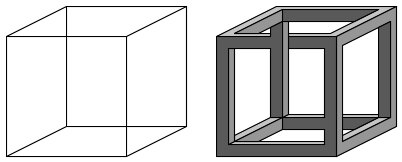
\includegraphics[width=0.8\textwidth]{figures/necker}
        %
\includegraphics[width=0.3\textwidth]{figures/face-vase}
        \vspace{-0.1cm}
        %\caption{Cube}
      \end{marginfigure}
      As binocular vision deepens and disambiguates, these notes may aid review
      of the lectures by offering a complementary, slightly more detailed
      organization of concepts.
      %
      \attn{You do not need to read these notes at all} to get an A
      in this course; conversely, \attn{you may not cite these notes} when
      solving homework or exams.
      %
      %You might enjoy skimming the appendice's three examples. 

  \samsection{A. Prologue} %in three examples}

    %\samsubsection{bird's eye framework}% data flow and goals 

        \begin{marginfigure}
          \vspace{+0.1cm}
          \par\noindent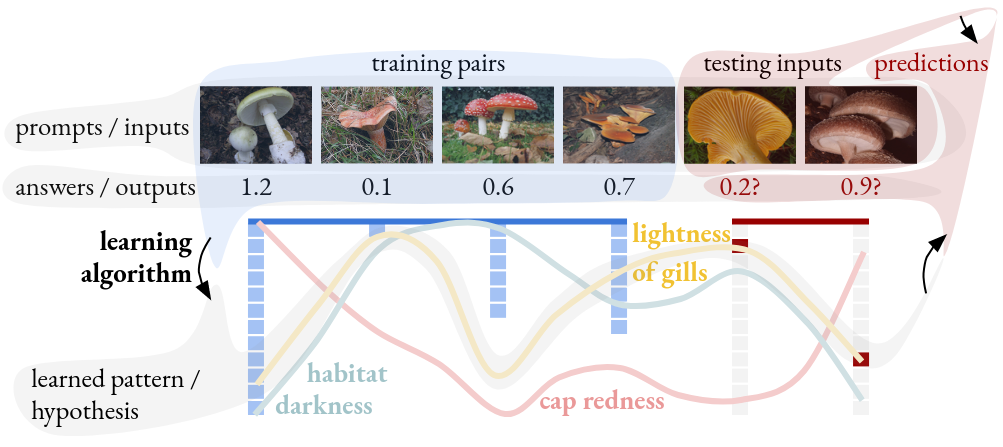
\includegraphics[width=\textwidth]{figures/supervised}\\
          We learn to predict poison levels of mushrooms from examples.  So we
            take a table of ``training'' examples as input and producing a
            ``pattern'' as output.  We evaluate the pattern on ``testing''
            prompts to make predictions.
          %\captionof{figure}{}
        \end{marginfigure}

    \samsubsubsection{kinds of learning}
      How do we communicate
      patterns of desired behavior?
      %new skills?
      %to other humans?  
      %
      %From most to least explicit,
      We can teach:
      \begin{description}
        \item[\textbf{by instruction}:  ]  ``to tell whether a mushroom is poisonous, first look at its gills...'' 
        \item[\textbf{by example}:      ]  ``here are six poisonous fungi; here, six safe ones.  see a pattern?''
        \item[\textbf{by reinforcement}:]  ``eat foraged mushrooms for a month; learn from getting sick.''
      \end{description}
      %
      Machine learning is the art of programming computers to learn from such
      sources.  
      We'll focus on the most important case: learning from examples (\S E shows how this case unlocks the others).
      %  key to the other modes of learning.).
      %\marginnote{%
      %  $\leftarrow$ We'll see in \S E that learning by example is
      %  key to the other modes of learning.
      %}
      %
      Given a list of $N$ examples of properly answered prompts, we
      seek a pattern: a map from prompts to answers.
      %In symbols,
      Say $\xX$ is the set of prompts; $\yY$, of answers.
      Then a program that learns from examples has type:\marginnote{%
        $\leftarrow$ We'll soon allow %account for
        uncertainty by letting
        patterns map to \emph{probability distributions} answers (\S B.1); then an
        example-based learner
        has type:\vspace{-0.15cm}
        $$\vspace{-0.15cm}
          \lL : (\xX\times \yY)^N \to (\xX\to \text{DistributionsOn}(\yY))
        $$
        %
        Sometimes, the prompt is always the same --- say,
        ``produce a beautiful melody'' --- and we seek (e.g.) to generate
        many answers. % and to learn a complicated distribution over the answers.
        %
        So-called \textbf{unsupervised learning}
        thusly focuses on output structure.
        \textbf{Supervised learning} focuses on the input-output
        relation.
        %
        %We won't take this probabilistic view until page 2. 
      }
      %\vspace{-0.1cm}
      $$\vspace{-0.1cm}
        \lL : (\xX\times \yY)^N \to (\xX\to \yY)
      $$
      %

    \samsubsubsection{learning error}
      Draw examples $\sS : (\xX\times \yY)^N$ %a list of examples
      from %nature's
      a distribution $\dD$ on $\xX\times
      \yY$. 
      A pattern $f:\xX\to \yY$
      has \textbf{training error}
      $
         \Ein(f) = \Pp_{(x,y)\sim \red{\sS}}[f(x)\neq y] 
      $
      %,
      %an average over examples;
      and \textbf{testing error}
      $
         \Eout(f) = \Pp_{(x,y)\sim \red{\dD}}[f(x)\neq y] 
      $.
      %,
      %an average over nature.
      %
      %We want $\lL$ to map $\sS$ to an $f$ with low $\Eout(f)$.\marginnote{%
      We want low $\Eout(\lL(\sS))$.\marginnote{%
        %  TODO: mention extereme class-imbalance and bayesian *decision* theory 
      }
      We often %define
      set $\lL$ to %roughly
      minimize $\Ein$ in a %over a
      candidates set $\hH \subseteq (\xX\to \yY)$.  Then $\Eout$
      decomposes
      into the failures
      of
      $\Ein$ to estimate $\Eout$, % (generalization),
      %of
      $\lL$ to minimize $\Ein$, and % (optimization), and 
      %of
      $\hH$ to contain ``the''
      %nature's
      truth: % (approximation): 
      \newcommand{\minf}[1]{{\inf}_{\hH}}
      \begin{align*}
          \Eout(\lL(\sS)) 
          =~&\Eout(\lL(\sS))      &-\,\,\,&      \Ein(\lL(\sS)) &~\}~& \text{\textbf{generalization} error} \\
          +~&\Ein(\lL(\sS))       &-\,\,\,& \minf{\hH}(\Ein(f)) &~\}~& \text{\textbf{optimization} error} \\
          +~&\minf{\hH}(\Ein(f))  &       &                     &~\}~& \text{\textbf{approximation} error}  
      \end{align*}
      These terms are in tension.  For example, as $\hH$ grows, the
      approx.\ error may decrease while the gen.\ error may
      increase --- this is the ``\textbf{bias-variance} tradeoff''.

      %In this page's final $2.5$cm we give a full example.
      \begin{marginfigure}
          \vspace{0.6cm}
          %
          \par\noindent
          Six example $(x,y)$s.  An $x$'s \emph{darkness} is its average
          pixel darkness; its \emph{width} is the stddev column index weighted
          by column darkness.  We normalize both to have max value $1.0$:\\ 
          \begin{tabular}{c}\hspace{-0.26cm}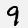
\includegraphics[width=0.14\textwidth]{example-mnist/mnist-trn-00}\\\hspace{-0.26cm}\red{$1$}\end{tabular}%
          \begin{tabular}{c}\hspace{-0.26cm}
\includegraphics[width=0.14\textwidth]{example-mnist/mnist-trn-01}\\\hspace{-0.26cm}\red{$1$}\end{tabular}%
          \begin{tabular}{c}\hspace{-0.26cm}
\includegraphics[width=0.14\textwidth]{example-mnist/mnist-trn-02}\\\hspace{-0.26cm}\cya{$0$}\end{tabular}%
          \begin{tabular}{c}\hspace{-0.26cm}
\includegraphics[width=0.14\textwidth]{example-mnist/mnist-trn-01}\\\hspace{-0.26cm}\red{$1$}\end{tabular}%
          \begin{tabular}{c}\hspace{-0.26cm}
\includegraphics[width=0.14\textwidth]{example-mnist/mnist-trn-04}\\\hspace{-0.26cm}\cya{$0$}\end{tabular}%
          \begin{tabular}{c}\hspace{-0.26cm}
\includegraphics[width=0.14\textwidth]{example-mnist/mnist-trn-05}\\\hspace{-0.26cm}\cya{$0$}\end{tabular}\\ 
          %
          %%We name the four plots below as $\offour{0},\offour{1},\offour{2},\offour{3}$. 
          %
          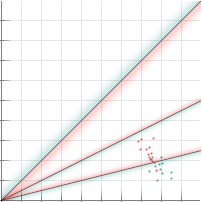
\includegraphics[width=0.48\textwidth]{example-mnist/train.png}%
          \hspace{0.03\textwidth}%
          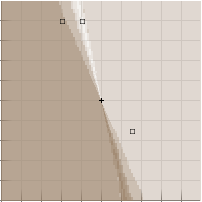
\includegraphics[width=0.48\textwidth]{example-mnist/train-scat.png}\\
          %
          %
          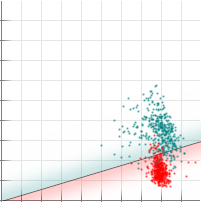
\includegraphics[width=0.48\textwidth]{example-mnist/test.png}%
          \hspace{0.03\textwidth}%
          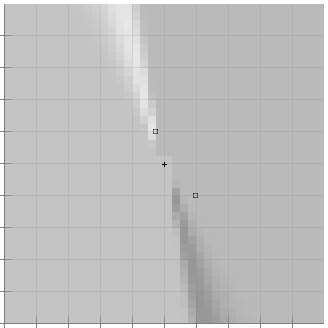
\includegraphics[width=0.48\textwidth]{example-mnist/test-scat.png}
          %
          Above: $3$ hypotheses classify $x$s in the darkness-width plane
          ($\offour{0}$).  The $(a,b)$ plane ($\offour{1}$) parameterizes
          linear hypotheses; darker means larger $\Ein$.
          $\offour{02}$'s axes range $[0, 0.5]$.
          $\offour{13}$'s axes range $[-99,+99]$; green indicates error $<0.1$.
          %
          $(a,b)=(-20,6)$
          minimizes $\Ein$ to $0.05$ but on fresh test samples ($\offour{2}$)
          suffers $\Eout=0.08$. 
      \end{marginfigure}
    \samsubsubsection{tiny example}
      $\xX = \{\text{grayscale~}28\!\times\!28\text{-pixel images}\}$; $\yY=\{{\cya{0}},{\red{1}}\}$. %,\cdots,9\}$.
      %Samples %$(x,y)$ from
      $\dD$'s samples are photos $x$ of 
      handwriting of the digit $y$. %handwriting of digit $y$. 
      %To sample from $\dD$, we ask a human to write digit $y\in \yY$, ask a human to write
      %that digit, and then photograph their writing.
      %
      %Each $x$ has a
      %width
      %and
      %darkness.
      %
      $\hH$ contains all ``linear hypotheses'' $f_{a,b}$ %:\xX\to\yY$ defined by
      defined by:
      $$
        f_{a,b}(x) = ~{\cya{0}} \text{~~if~~} a\cdot \text{width}(x) + b\cdot\text{darkness}(x) < 0 \text{~~else~~} {\red{1}} 
      $$ 
      Our program $\lL$ loops over all integer pairs $(a,b)$ in $[-99,+99]$ to
      minimize $\Ein$, giving $(a,b)=(-20,6)$ with $\Ein \approx 5\%$.  We
      got optimization error $\approx 0$ (albeit by \emph{unscalable
      brute-force}).  So approximation error $\approx \Ein \approx 5\%$.
      Indeed, our straight lines are \emph{too simple}: width and darkness lose
      useful information and the ``true'' boundary looks curved (see $\offour{0}$'s curve).
      %
      The testing error $\Eout \approx 8\%$ exceeds $\Ein$: we suffer
      \emph{generalization error}.
      %% actually approx error should be measured on the train set, which ain't that bad
      %
      In 6.86x we'll address all three italicized issues.

      \attn{Exercise:} {how do $\offour{0}$'s two straight lines and
      $\offour{1}$'s two marked points correspond?}
      %
      \attn{Exercise:} {visualize $\Ein(f_{a,b})$ in the $(a,b)$ plane for
      $N=1$ training example.}
      %
      \attn{Exercise:} {why is generalization error usually positive?}

%==============================================================================
%=====  2.  LINEAR MODELS  ====================================================
%==============================================================================

  \newpage
  \samsection{B. Linear models}
    \samsubsection{0. linear approximations} 
      \samquote{
        He had bought a large map representing the sea, \\
        Without the least vestige of land: \\
        And the crew were much pleased when they found it to be \\
        A map they could all understand.
      }{charles dodgson}
      \samsubsubsection{featurization}  % as an art of 
        As in the prologue, we represent our input $x$ as a fixed-length list
        of numbers so that we can treat $x$ with math.  There,
        we represented each photograph by $2$ numbers: width and
        darkness.  We could instead have represented each photograph by $784$
        numbers, one for the brightness at each of the $28\cdot 28=784$ many
        pixels.  Or by $10$ numbers, each measuring the overlap of $x$'s
        ink with a ``standard'' photo of the digits $0$ through $9$.

        When we choose how to represent $x$ by a list of numbers, we're
        choosing a \textbf{featurization}.  We call each number a ``feature''.
        For example, width and darkness are two features.

        %``width'' and ``darkness'' are \emph{features}: maps $\xX\to \Rr$ used
        %to pre-process $x$s.

        \attn{TODO: mention one-hot, etc}
        \attn{TODO: mention LOWRANK for multiregression? (relevant to futrure intermezzo?}
        %
        There are lots of interesting featurizations, each making different
        patterns easier to learn.  So we judge a featurization with respect to
        the kinds of patterns we use it to learn.
        \attn{TODO: graphic of separability; and how projection can reduce it}
        Learning usually happens
        more accurately, robustly, and interpretably when our featurization is
        abstract (no irrelevant details) but complete (all relevant details),
        compressed (hard to predict one feature from the others) but accessible
        (easy to compute interesting properties).


        \attn{Exercise:} {Beyond width and darkness, what features do you think
        might help us to separate digits $0$ from $1$ by a line through the origin?  How about $3$ from $8$?}


      \samsubsubsection{geometry of feature-space} % pictures!

        Caution: a feature $A(\sfx)$ that is statistically independent from
        $\sfy$ may still be relevant for predicting $\sfy$.\marginnote{%
          Example.  Consider the uniform distribution on the four corners of a
          tetrahedron embedded within the corners of a cube \attn{TODO:
          graphic}.  The three spatial coordinates give three bit-valued random
          variables.  Any two of these variables are independent.  But the
          three together are dependent.
          \attn{TODO: also do a decision boundary (simpsons style) graph
          illustrating this phenomenon}
        }
        For example, if
        $A, B$ are two features, it is possible that $A(\sfx), \sfy$ are
        independent and that $B(\sfx), \sfy$ are independent and yet
        $A(\sfx),B(\sfx), \sfy$ are \emph{dependent}!

        \attn{TODO: example featurization (e.g. MNIST again?)}

        \attn{TODO: projectivization (say this foreshadows kernel discussion?)}

        Now say we've decided on a \textbf{featurization} of our input
        data $x$.
        $$
          f_{a,b}(x) = ~0 \text{~~if~~} a\cdot \text{width}(x) + b\cdot\text{darkness}(x) < 0 \text{~~else~~} 1 
        $$ 

        \attn{Illustrate `averaging' of good features vs `correction' of one feature by another (how much a feature correlates with error)}

      \samsubsubsection{linear algebra} % vectors and co-vectors
        Linear algebra is the part of geometry that focuses on %the notions of
        when a point is the origin, when a `line' is a straight, and when two
        straight lines are parallel.
        %
        Linear algebra thus helps us deal with the preceding pictures\marginnote{%
          $\leftarrow$ It is important to \attn{thoroughly understand these
          basics} of linear algebra.  Please see \S G.2 for further discussion
          of these basics. 
        }
        mathematically.  The concept of `straight lines' gives a simple,
        flexible model for extrapolation from known points to unknown points.
        That is intuitively why linear algebra will be crucial at every stage
        of 6.86x.

        The elements of linear algebra are \textbf{column vectors} and
        \textbf{row vectors}.  \attn{FILL IN}
        Though we represent the two similarly in a
        computer's memory, they have different geometric meanings.
        We save 
        much anguish by remembering the difference.  \attn{FILL IN}

        \attn{FILL IN LINEAR DECISION BOUNDARY! (remark on featurization and
        argmax nonlinearities)}

        We may \textbf{evaluate} a row vector on a column vector.  \attn{FILL
        IN} A \textbf{dot product} is a way of translating between row and
        column vectors.  \attn{FILL IN: DISCUSS GENERALIZATION; (DISCUSS ANGLE, TOO)}

        \attn{FILL IN COMPUTATION AND BASES}

        \attn{VISUAL ILLUSTRATION OF HOW CHOICE OF DOT PRODUCT MATTERS}

      \samsubsubsection{richer outputs}%larger $\yY$s} % $k$-ary classification; regression; probabilities
        We've learned how to construct a set $\hH$ of candidate patterns 
        $$
          f_{\vec w}(\vec x) = \text{threshold}(\vec w\cdot \vec x) 
        $$
        that map (a featurization of) a prompt $\vec x$ to a binary answer $y=0$ or $y=1$.

        What if we're interested in predicting a richer kind of $y$?  For
        example, maybe there are $k$ many possible values for $y$ instead of
        just $2$.  Or maybe there are infinitely many possible values --- say,
        if $y$ is a real number or a length-$l$ list of real numbers.  Or maybe we want the added nuance of
        predicting probabilities, so that $f$ might output ``20\% chance of
        label $y=0$ and 80\% chance of label $y=1$'' instead of just ``$y=1$''.

        I'll write formulas and then explain.
        $$
          f_{\vec w_i : 0\leq i < k}(\vec x) = \text{argmax}_i(\vec w_i\cdot \vec x) 
        $$
        $$
          f_{\vec w}(\vec x) = \vec w \cdot \vec x
        $$
        \attn{TODO: add multi-output regression?}
        $$
          f_{\vec w_i  : 0\leq i < k}(\vec x) = \text{normalize}(\exp(\vec w_i \cdot \vec x) : 0\leq i < k)
        $$
        \attn{TODO: interpret}

        \attn{TODO: discuss measures of goodness!}

        \attn{TODO: talk about structured (trees/sequences/etc) output!}

        \newpage
    \samsubsection{1. iterative optimization} 
      \samquote{
        Hey Jude, don't make it bad \\
        Take a sad song and make it better \\
        Remember to let her under your skin \\
        Then you'll begin to make it \\
        Better, better, better, better, better, better, ...
      }{paul mccartney, john lennon}

      %There are two routes toward reading this subsection.
      %
      %%  You can \attn{read the passages on ``perceptrons'' and on
      %%  ``logistic models'' in either order}; it depends on
      %%  your personality.  Logistic models and perceptrons are two sides of
      %%  the same coin.  The former is continuous; the latter, discrete.
      %%  I prefer to read ``logistic models'' first.

      \samsubsubsection{(stochastic) gradient descent}
        We have a collection $\hH$ of candidate patterns together with a
        function $1-\Ein$ that tells us how good a candidate is.\marginnote{%
          $\leftarrow$ We view $1-\Ein$ as an estimate of our actual notion of ``good'': $1-\Eout$.
        }
        %
        In \S A we found a best candidate by brute-force search over all of
        $\hH$; this doesn't scale to our linear models, since now $\hH$ is
        intractably large.
        %
        So: \emph{what's a faster algorithm to find (or approximate) a best candidate?}

        A common idea is to start arbitrarily with some $h_0\in \hH$ and
        repeatedly improve to get $h_1, h_2, \cdots$.  Two questions are:
        \emph{how do we select $h_{t+1}$ in terms of $h_t$}?  And \emph{how do
        we know when to stop}?  We'll discuss termination conditions later
        --- for now, let's agree to stop at $h_{1000}$.   

        As for selecting a next candidate, we'd like to use more detailed
        information on $h_t$'s inadequacies to inform our proposal $h_{t+1}$.
        Intuitively, if $h_t$ misclassifies a particular $(x_n, y_n) \in \sS$,
        then we'd like $h_{t+1}$ to be like $h_t$ but nudged a bit in the
        direction of accurately classifying $(x_n, y_n)$.

        %
        \attn{FILL IN FOR PROBABILITIES (LOGISTIC) MODEL} 

        This is the idea of \textbf{gradient descent}.
        \attn{MOTIVATE AND GIVE PSEUDOCODE FOR STOCHASTIC GD} 
        
      \samsubsubsection{logistic models} %``soft''

        \attn{mention convexity and convergence?}

      \samsubsubsection{perceptrons} %as constrained logistic regression; ``hard''
        We get a historically crucial and intuition-pumping algorithm when we
        do logistic regression in the limit of low temperatures.

        \attn{mention convergence?}
        \attn{show trajectory in weight space over time -- see how certainty degree of freedom is no longer redundant? (``markov'')}

      \samsubsubsection{hinge loss and svms}
        Logistic ain't the only way to go in classification.  Here we discuss
        a generalization and the merits of various special cases.

        We may view logistic regression as minimizing
        $$
          \sum_i \log(1+\exp(-y_i\vec w\cdot \vec x_i))
          =
          \sum_i \text{softplus}(-y_i\vec w\cdot \vec x_i) 
        $$
        Here, $\text{softplus}$ is our name for a function that sends
        $z$ to $\log(1+\exp(z))$.

        Three essential properties of $\text{softplus}$ are that:
        (a) it is convex
        (b) it upper bounds the step function. 
        (b) it is non-decreasing for inputs in $[-1,+1]$.

        We could replace $\text{softplus}$ by $\text{hinge}$ or
        $\text{hinge}^2$ or $\text{parab}$ or $\text{hyper}$ or other
        functions with properties (a),(b),(c).

        Here, $\text{hinge}(z) = \text{max}(0,z+1)$.
        Here, $\text{parab}(z) = (z+1)^2$.
        Here, $\text{hyper}(z) = \text{avg}(z, \sqrt{z^2+4})$.
        Here, $\text{poled}(z) = 1/(\text{min}(z,1)-1)$.

        \attn{probabilistic interpretations; tails}

        \attn{response to outliers}

        \attn{support vectors}

      \newpage
    \samsubsection{2. priors and generalization} 
      \samquote{
        I believe that either Jupiter has life or it doesn't.
        But I neither believe that it does, nor do I believe that it doesn't.
      }{raymond smullyan}
      \samsubsubsection{on overfitting}
      \samsubsubsection{log priors and bayes}
      \samsubsubsection{$\ell^p$ regularization; sparsity} % eye regularization example!
      \samsubsubsection{estimating generalization}

      \newpage
    \samsubsection{3. model selection} 
      \samquote{
        All human beings have three lives: public, private, and secret.
      }{gabriel garc\`ia marquez}
      \samsubsubsection{taking stock so far}
      \samsubsubsection{grid/random search}
      \samsubsubsection{selecting prior strength}
      \samsubsubsection{overfitting on a validation set}

      \newpage
    \samsubsection{4. generalization bounds} 
      \samquote{
        A foreign philosopher rides a train in Scotland.  Looking out the window,
        they see a black sheep; they exclaim: ``wow!  at least one side of one sheep is black in Scotland!'' 
      }{unknown}
      %\samquote{
      %  An engineer, a statistician, and a philosopher are riding a train through Scotland.
      %  They look out the window and sees a black sheep.
      %  The engineer exclaims, ``Hey!  In Scotland the sheep are black!''
      %  The statistician corrects the engineer: ``Strictly speaking, all we know is that there's at least one black sheep in Scotland.''
      %  The philosopher chimes in: ``Strictly speaking, all we know is that is that at least one side of one sheep is black in Scotland.''
      %}{unknown}
      \samsubsubsection{dot products and generalization}
      %\samsubsubsection{perceptron bound}
      \samsubsubsection{dimension bound}
      \samsubsubsection{margin bound}
      \samsubsubsection{bayes and testing} % PAC Bayes?  testing Sets?  or maybe testing sets should be part of model selection

      \newpage
    \samsubsection{5. ideas in optimization} 
      \samquote{
        premature optimization is the root of all evil
      }{donald knuth}
      \samsubsubsection{local minima} % convexity, initialization}
      \samsubsubsection{implicit regularization}
      \samsubsubsection{learning rate schedule}
      \samsubsubsection{learning rates as dot products} % connects to whitening / pre-conditioning; ties into next subsection on kernels

      \newpage
    \samsubsection{6. kernels enrich approximations} 
      \samquote{... animals are divided into (a) those
        belonging to the emperor; (b) embalmed ones; (c) trained ones; (d)
        suckling pigs; (e) mermaids; (f) fabled ones; (g) stray dogs; (h) those
        included in this classification; (i) those that tremble as if they were
        mad; (j) innumerable ones; (k) those drawn with a very fine camel hair
        brush; (l) et cetera; (m) those that have just broken the vase; and (n)
        those that from afar look like flies.
      }{jorge luis borges}
      \samsubsubsection{features as pre-processing} % start with example of (x \mapsto (1, x)) bias trick!
      \samsubsubsection{abstracting to dot products} % mention mercer but don't emphasize
      \samsubsubsection{kernelized perceptron and svm} % also gaussian process regression?
      \samsubsubsection{kernelized logistic regression} % leads to nonlinearities...

%%%%%%%%%%%%%%%%%%%%%%%%%%%%%%%%%%%%%%%%%%%%%%%%%%%%%%%%%%%%%%%%%%%%%%%%%%%%%%%

  \newpage
  \samsection{An Intermezzo}
    Congrats!  If you've digested all the above, then you've digested by far
    the most important part of these notes.
    %
    I invite you to take a break, make a sandwich, drink some coffee, enjoy
    a walk, before proceeding.

    To accompany your break, below is some poetry generated by a rudimentary
    language model.  You'll be able to completely understand how it works; that
    said, it doesn't work well.  The tools of the next section can drastically
    improve this model.

    \samsubsubsection{Method}


    \samsubsubsection{Output}

%==============================================================================
%=====  3.  NONLINEARITIES  ===================================================
%==============================================================================

  \newpage
  \samsection{C. Nonlinearities}
    \samsubsection{0. fixed featurization} 
      \samquote{
        Doing ensembles and shows is one thing, but being able to front a
        feature is totally different.  ...  there's something about ... a
        feature that's unique. 
      }{michael b.\ jordan}
      \newpage
    \samsubsection{1. learned featurizations} 
      \newpage
    \samsubsection{2. differentiation} 
      \newpage
    \samsubsection{3. architecture and symmetry} 
      \samquote{
        About to speak at [conference]. Spilled Coke on left leg of jeans, so poured some water on right leg so looks like the denim fade.
      }{tony hsieh}
      \newpage
    \samsubsection{4. feature hierarchies} 
      \newpage
    \samsubsection{5. stochastic gradient descent} 
      \samquote{
        The key to success is failure.
      }{michael j.\ jordan}

      \newpage
    \samsubsection{6. loss landscape shape} 
      \samquote{
        The virtue of maps, they show what can be done with limited space, they foresee that everything can happen therein.
      }{jos\'e saramago}

%%%%%%%%%%%%%%%%%%%%%%%%%%%%%%%%%%%%%%%%%%%%%%%%%%%%%%%%%%%%%%%%%%%%%%%%%%%%%%%

  \newpage
  \samsection{An Intermission}
    Congrats!  If you've digested all the above, then you've digested by far
    the most important part of these notes.
    %
    I invite you to take a break, make a sandwich, drink some coffee, enjoy
    a walk, before proceeding.

    To accompany your break, below is some poetry generated by a rudimentary
    language model.  You'll be able to completely understand how it works; that
    said, it doesn't work well.  The tools of the next section can drastically
    improve this model.

%==============================================================================
%=====  4.  STRUCTURED INFERENCE  =============================================
%==============================================================================

  \newpage
  \samsection{D. Structured inference}
    \samsubsection{0. graphical generative models} 
      \samquote{
        ... [to treat] complicated systems in simple ways[,] probability ...
        implements two principles[:] [the approximation of parts as
        independent] and [the abstraction of aspects as their averages].
      }{michael i.\ jordan}

      \newpage
    \samsubsection{1. inferring conditional marginals} 
      \newpage
    \samsubsection{2. learning the parameters} 
      \newpage
    \samsubsection{3. hierarchy and mixtures} 
      \samquote{
        I like crossing the imaginary boundaries people set up between different fields --- it's very refreshing.
      }{maryam mirzakhani}
      \newpage
    \samsubsection{4. hierarchy and transfer} 
      \newpage
    \samsubsection{5. variational and sampling methods} 
      \samquote{
        Take a chance, won't you?
        Knock down the fences that divide.
      }{thurgood marshall}
      \newpage
    \samsubsection{6. amortized inference} 
      \samquote{
        Reminding myself that I have a tailbone keeps me in check.
      }{tig notaro}

%%%%%%%%%%%%%%%%%%%%%%%%%%%%%%%%%%%%%%%%%%%%%%%%%%%%%%%%%%%%%%%%%%%%%%%%%%%%%%%

  \newpage
  \samsection{A Divertisment}
    Congrats!  If you've digested all the above, then you've digested by far
    the most important part of these notes.
    %
    I invite you to take a break, make a sandwich, drink some coffee, enjoy
    a walk, before proceeding.

    To accompany your break, below is some poetry generated by a rudimentary
    language model.  You'll be able to completely understand how it works; that
    said, it doesn't work well.  The tools of the next section can drastically
    improve this model.

%==============================================================================
%=====  5.  REDUCTIONS TO SUPERVISION  ========================================
%==============================================================================

  \newpage
  \samsection{E. Reductions to supervision}

    \samsubsection{0. to build a tool, use it} 
      \samquote{
        We are what we pretend to be, so we must be careful about what we pretend to be.
      }{kurt vonnegut}

      \newpage
    \samsubsection{1. distributions as maps} 
      \samquote{
        For me, sampling is a high art.
        Most people don't see it that way, but it's a beautiful thing.
        I wouldn't know anything about music if it wasn't for samples.
      }{barrington hendricks}
      %\samquote{
      %  Possession of anything new or expensive only reflected a person's lack of
      %  theology and geometry; it could even cast doubts upon one's soul.
      %}{john toole}

      \newpage
    \samsubsection{2. self-supervised: downstream tasks} 
      \samquote{
        Find out who you are and do it on purpose.
      }{dolly parton}
      %\samquote{
      %  Be a pattern to others and then all will go well.
      %}{marcus cicero}

      \newpage
    \samsubsection{3. self-supervised: autoregression} 
      \samquote{
        When we learn to speak, we learn to translate.
      }{octavio paz}

      %\samquote{
      %  for last year's words belong to last year's language \\
      %  and next year's words await another voice
      %}{thomas eliot}
      %\samquote{
      %  To love is to undress our names.
      %}{octavio paz}

      \newpage
    \samsubsection{4. reinforcement: exploration-exploitation} 
      \samquote{
        We're all curious about what might hurt us.
      }{frederico garc\'ia lorca}

      \newpage
    \samsubsection{5. reinforcement: states and $q$-values} 
      \samquote{
        There's a good reason why nobody studies history: it just teaches you
        too much.
      }{noam chomsky}

      \samsubsubsection{on-policy learning}
      \samsubsubsection{off-policy learning}
      \samsubsubsection{deep curricula: re-play}
      \samsubsubsection{deep curricula: self play}
      \samsubsubsection{the deadly triad}

      \newpage
    \samsubsection{6. beyond the i.i.d.\ hypothesis}
      \samquote{
        When I was a boy of 14, my father was ignorant; I could hardly stand to
        have the old man around. But when I got to be 21, I was astonished at
        how much the old man had learned in seven years.
      }{mark twain}
      \samsubsubsection{out-of-distribution tests}
      \samsubsubsection{dependent samples}
      \samsubsubsection{causality}

%%%%%%%%%%%%%%%%%%%%%%%%%%%%%%%%%%%%%%%%%%%%%%%%%%%%%%%%%%%%%%%%%%%%%%%%%%%%%%%

  \newpage
  \samsection{A Farewell}
    Congrats!  If you've digested all the above, then you've digested by far
    the most important part of these notes.
    %
    I invite you to take a break, make a sandwich, drink some coffee, enjoy
    a walk, before proceeding.

    Congrats!  
    \samsubsubsection{Further Reading}

%==============================================================================
%=====  7.  APPENDICES  =======================================================
%==============================================================================

  \newpage
  \samsection{Appendices}
    Here are ``refreshers'' on programming and on math, especially on the math
    of high dimensions and of bayes' law.  Beyond establish our naming
    conventions, they can help jog your memory of the math and programming you
    might have encountered prior to taking 6.86x.\marginnote{%
      %%Depending on your background and personality, you might recognize and
      %%care that throughout these notes we are a bit sloppy with our probability
      %%and programming.  No standard compiler can compile our pseudocode;
      %%likewise, our theorems are actually theorem sketches in need of
      %%additional analytic hypotheses. 
      %%%
      %%For readers so concerned, we assume an additional prerequisite: enough
      %%technical background that we may leave implicit both the articulation of
      %%measure-theory technicalities and the implementation of pseudocode.
    }
    %
    The refreshers are meant neither to explain their content well nor to
    provide a complete outline of skills needed for 6.84x.  For further
    support, please \attn{ask questions on the forum} and \attn{make frequent
    use of office hours}!

    \samsubsection{python programming refresher}
      \samquote{
        If I have not seen as far as others, it is because giants were standing on my shoulders.
      }{hal abelson}

      \samsubsubsection{setup}
        Python is a popular programming language.  Beyond the Python
        interpreter, there is an ecosystem of useful tools: machine learning
        modules that help us avoid reinventing the wheel; a rainbow of
        feature-rich IDEs to choose from; and a package manager called
        \texttt{conda} that eases the dependency-spaghetti hassle often
        present in installing the right version of stuff.  

        Let's set up Python3.

        I'll assume we're working on Linux
        (specifically, Ubuntu 20 or related).  If you're on a different Linux
        or on MacOS, then similar steps should work --- google search to figure
        out how.  If you're on Windows 10 or higher, then similar steps should
        work after you set up the ``Linux Subsystem for Windows.''

        \attn{FILL IN: how to run, comments, basic stdIO}
        \attn{line by line HELLO WORLD; string type}
        \attn{line by line FAHRENHEIT KELVIN CELSIUS; float and integer types}

      \samsubsubsection{state and control flow}
        % use-mention distinction; syntax-semantic.s  Asimov ROBOT

        \attn{finite state automata; skip, abort}
        \attn{variable cube; assignment}
        \marginnote{%
          Once you learn how to program, I highly recommend reading Edsger
          Dijkstra's \emph{A Discipline of Programming}.  That book contains
          many beautiful viewpoints that made me a better programmer.
        }
        %
        \attn{sequencing}
        \attn{conditionals} % also mention trivalent CHOICE operator?  
        \attn{iteratives}
        \marginnote{%
          % for-range idiom; break, continue, else in loops 
        }
        \attn{nesting, (scope?,) indentation}

      \samsubsubsection{routines}
        %\attn{mention SCOPE somewhere (perhaps earlier than this passage?)}
        \attn{lambdas}
        \attn{\texttt{def}d functions (ordinary args, return)}
        \attn{interfaces: (kwargs; None as default return value; sentinels; more)}
        \attn{code architecture and hygiene}
      \samsubsubsection{data in aggregate}%container structures}
        \attn{lists and numpy arrays} % no tuples
        \attn{dictionaries} % no sets; mention cacheing (and hence also global scope??)
        \attn{comprehensions}
        \attn{functional idioms}
      \samsubsubsection{input/output}
        \attn{print formatting and flushing}
        \attn{basic string manipulations (strip, join, etc)}
        \attn{file io}
        \attn{command line arguments}
        \attn{example: read csv}
        %
        \attn{random generation and seeds??}
      \samsubsubsection{how not to invent the wheel} %modules: os, numpy, matplotlib}
        \attn{matplotlib.plot}
        \attn{numpy}
        \attn{os}
        \attn{package managers etc}
      \samsubsubsection{arrays aka tensors}
        \attn{}
        \attn{}
        \attn{}
        \attn{}

    %\samsubsection{math notation and refresher}
    \samsubsection{probability refresher}
      We've tried to use 
        \vspace{-0.10cm}
      $$
        \text{\textsf{sans serif} for the names of random variables,}
        \vspace{-0.15cm}
      $$
      $$
        \text{\emph{italics} for the values they may take, and}
      $$
      $$
        \text{$\mathcal{CURLY~CAPS}$ for sets of such values.} 
      $$
      For example, we write $p_{\sfy|\sfh}(y|h)$ for the probability that the
      random variable $\sfy$ takes the value $y$ conditioned on the event that
      the random variable $\sfh$ takes the value $h$.
      %
      Likewise, our notation $p_{\hat \sfh|\sfh}(h|h)$ indicates the
      probability that the random variables $\hat \sfh$ and $\sfh$ agree in
      value given that $\sfh$ takes a value $h\in \hH$.

    \samsubsection{linear algebra refresher}
      \samquote{
        Stand firm in your refusal to remain conscious during algebra.
        In real life, I assure you, there is no such thing as algebra.
      }{fran lebowitz}

      Linear algebra is the part of geometry that focuses on %the notions of
      when a point is the origin, when a `line' is a straight, and when two
      straight lines are parallel.
      %
      Linear algebra thus helps us deal with the preceding pictures\marginnote{%
        $\leftarrow$ It is important to \attn{thoroughly understand these
        basics} of linear algebra.  Please see \S G.2 for further discussion
        of these basics. 
      }
      mathematically.  The concept of `straight lines' gives a simple,
      flexible model for extrapolation from known points to unknown points.
      That is intuitively why linear algebra will be crucial at every stage
      of 6.86x.

      The elements of linear algebra are \textbf{column vectors} and
      \textbf{row vectors}.  \attn{FILL IN}
      Though we represent the two similarly in a
      computer's memory, they have different geometric meanings.
      We save 
      much anguish by remembering the difference.  \attn{FILL IN}

      \attn{FILL IN LINEAR DECISION BOUNDARY! (remark on featurization and
      argmax nonlinearities)}

      We may \textbf{evaluate} a row vector on a column vector.  \attn{FILL
      IN} A \textbf{dot product} is a way of translating between row and
      column vectors.  \attn{FILL IN: DISCUSS GENERALIZATION; (DISCUSS ANGLE, TOO)}

      \attn{FILL IN COMPUTATION AND BASES}

      \attn{VISUAL ILLUSTRATION OF HOW CHOICE OF DOT PRODUCT MATTERS}


    \newpage
    \samsubsection{mathematical language refresher}
      \samquote{
          \begin{flushleft}
          \texttt{\phantom{}def get\_random\_number():} \\
          \texttt{\phantom{....}return 4 \# chosen by a fair dice roll} \\
          \texttt{\phantom{.............}\# guaranteed to be random}
          \end{flushleft}\phantom{.}
      }{randall munroe, translated by sam to Python}

      \samsubsubsection{space} %and coordinates}
        Ren\'e Descartes had a good idea: we can study the invisible and
        intangible by hacking our visual cortex and our proprioceptive senses.
        %
        We do this through the profound metaphor of \textbf{SPACES of BLAH},
        where BLAH is some kind of thing we're analyzing

        In the next two passages, we discuss two mental moves we like to do
        with this spatial metaphor.  The first simplifies our thinking by
        forgetting irrelevant truths.  The second simplifies our thinking by
        positing useful falsehoods.
      \samsubsubsection{sameness} % abstraction
        The key challenges here are of \emph{uniqueness} and \emph{lifting} 
      \samsubsubsection{specialness} % approximation
        The key challenges here are of \emph{existence} and \emph{extension} 
      %
      \samsubsubsection{types}
        In technical subjects, it is very useful to keep track of what ``types''   
        our objects of study are.  This reduces cognitive load by reminding
        us what we're allowed to do with the objects.

        We write ``$x:S$'' (or, synonymously, ``$x\in S$'')\marginnote{%
          $\leftarrow$ In many math books the two are not synonymous.  But this
          ain't a math book.
        } as shorthand for
        the sentence: \emph{the thing we're calling $x$ has the type we're
        calling $S$.}


        We can build new types from old through: if $X,Y$ are two types, then
        $X\sqcup Y$ names the type of things that are either of type $X$ or
        of type $Y$.  Meanwhile, $X\times Y$ names the type of pairs $(x,y)$
        where $x:X$ and $y:Y$.  Finally, $X\to Y$ names the type of functions
        from $X$ to $Y$.  So $f:X\to Y$ means that $f$ has type $X\to Y$.
        %The operations of $\sqcup, \times, \to$ are analogous to addition,
        %multiplication, and (reverse) exponentiation of natural numbers. 

        We have functions
        $\text{left}:X\to (X\sqcup Y)$ and $\text{right}:Y\to (X\sqcup Y)$ 
        and
        $\text{first}:(X\times Y)\to X$ and $\text{second}:(X\times Y)\to Y$.

        We have 
            $\text{left}(x) : X\sqcup Y$ if and only if $x:X$
            and
            $\text{right}(y) : X\sqcup Y$ if and only if $y:Y$.
        We have $z : X\times Y$ if and only if $\text{first}(z):X$ and
        $\text{second}(z):Y$.

        We often consider natural numbers as types; the natural number $n$,
        when viewed as a type, has exactly $n$ many elements.  Thus,
        $X\sqcup 1$ is a type of things that are either members of $X$ or
        the unique member of $1$.

      \samsubsubsection{transforms} % functions
        When a mathematician says ``\textbf{function}'', they are
        talking about a gigantic (often infinitely large) table of input-output
        pairs.  The table assigns to each input exactly one output.

        There are infinitely many functions.  One example is
        $$
            f: \Rr\to\Rr \text{~defined by~} x \mapsto x^2
        $$
        The above line of math is standard short-hand for the following
        paragraph:\\
        \indent\emph{Consider a big table of input-output pairs.  Each input is a real
        number.  Each output is a real number.  If $x$ is a real number, then
        there is exactly one input-output pair whose input is $x$.  Moreover,
        the output of that pair is the real number $x^2$.  We'll call this big
        table ``$f$''.  We'll write ``$f(x)$'' to refer to the output
        corresponding to an input $x$; in this case, $f(x)$ is another name for
        $x^2$.  For example, $f(5)$ is $25$.}

      \samsubsubsection{tuples and tags} % products and coproducts

    \newpage
    \samsubsection{calculus refresher}
      %\samquote{
      %  The self is not something ready-made, but something in continuous
      %  formation through choice of action.
      %}{john dewey}
      \samsubsubsection{derivatives}
        When we find the \emph{derivative} of a function, we're finding a
        best linear approximation to that function near a point on that
        function's graph.  
        %
        Said another way, a derivative $D(f)(x)$ of a function $f$ at an
        input $x$ is a linear function $h \mapsto D(f)(x)(h)$ such that
        $$
          f(x+h) \approx f(x) + D(f)(x)(h) 
          \text{~for all small~} h, 
          \text{~for all~} x 
        $$

        For example, if $f(x)=1+3x$ then $D(f)(x)$ is the map $h\mapsto 3h$. 
        If $f(x)=x^2$ then $D(f)(x)$ is the map $h\mapsto 2x\cdot h$. 
        \begin{marginfigure}
            \attn{TODO}: perimeter graphic for $x^2$'s derivative
        \end{marginfigure}

        \attn{DISCUSS} Linearity in $f$

        \attn{DISCUSS Chain Rule}

        \attn{DISCUSS Product Rule}

      \samsubsubsection{minima}
      \samsubsubsection{exponential function}%differential equations}
        Much as we might try to solve ``algebraic equations'' (if $y^3 + y =
        t^2 + 1$, what is $y$ in terms of $t$?), we sometimes also want to
        solve ``differential equations'' (if $D y = - t \cdot y$, what is $y$
        in terms of $t$?). 

        From the world of algebraic equations, we might expect two subtleties:

        (a) sometimes, we won't be able to write the answer in terms of the
        familiar arithmetic operations of addition, subtraction,
        multiplication, and division; what we do instead is to express the
        answers to a diversity of harder problems in terms of answers to a few
        easier problems. 
        %
        For example, $y^2=t$ has no ``arithmetic'' solution;
        instead, we just give a name (``$\text{sqrt}$'') to that function.  We
        can solve more complicated equations, e.g.\ $y^2=t+y$, using the
        arithmetic operations together with $\text{sqrt}$.  This re-expression
        may seem like cheating; its upshot is that by building intuition for
        the one new function $\text{sqrt}$, we end up getting insight into lots
        of more complicated equations.
        %
        In the world of differential equations, we likewise introduce a few
        new functions.  The most important is called \textbf{the exponential
        function}, or $\text{exp}$ for short.  Just as
        $\text{sqrt}$ is defined to solve $y^2=t$, our function $\text{exp}$
        is defined to solve $Dy = y$.

        (b) sometimes, there are multiple solutions.  For example, both
        $\text{sqrt}(5)$ and $-\text{sqrt}(5)$ solve $y^2=5$.  What we do in algebra is to
        choose one kind of solution as the thing we give a name to, and we
        remember a simple rule for how all the other solutions relate to this
        standard one.  Thus, we define $\text{sqrt}$ as the continuous solution
        to $y^2=t$ \emph{that at input one has output one}:
        $y(1)=1$.\marginnote{%
          This definition works just as well: $\text{sqrt}$ is the solution to
          $y^2=t$ \emph{that's always at least zero}.
        } We get the other solution if we
        scale the output by $-1$.
        %
        In the world of differential equations, there is a similar ambiguity.
        If $y=\text{exp}(t)$ solves $D y = y$, then so does $y=2\cdot
        \exp(t)$: we can scale the output by any number to get another
        solution.  We address this scaling ambiguity by defining $\exp$ as the
        solution to $D y = y$ \emph{that at input zero has output one}:
        $y(0)=1$.  We get the other solutions if we scale the output.

        Okay, so that's our golden definition:\marginnote{%
          \attn{INSERT graph of $\exp$}
          \attn{Give a sense of scale: what is $\exp$ at $-10,-2.3,-0.69,-1,0,+1,+0.69,+2.3,+10$?}
        }
        $$
          D \exp(t) = \exp(t)
          \quad \quad
          \exp(0) = 1
        $$
        All solutions of $D y = t$ are multiples of this solution.

        From the previous paragraph flow three facts about $\exp$ that'll help
        us in 6.86x.  Here they are, with non-standard and suggestive names:

        (a) Entropy Law 
        $$
          \exp(a+b) = \exp(a)\cdot\exp(b)
        $$
        To see this fact, just note that we can horizontally shift $\exp$'s
        graph by, says, $5$ to get the graph of a function defined by
        $t\mapsto \exp(5+t)$.  Since derivatives are just best linear
        approximations, and since a graph's best linear approximations simply
        shift along with the graph, we have $D \exp(5+t) = \exp(5+t)$.  So 
        this shifted function \emph{also} solves $D y = y$.  Therefore,
        it must be a multiple of our standard solution $\exp$.  Which multiple?
        Well, at $t=0$ we have $\exp(5+t)=\exp(5)$ while $\exp(t)=1$.  So we
        want to scale $\exp(t)$ by the number $\exp(5)$ to get $\exp(5+t)$.
        We conclude:
        $$
          \exp(5+t) = \exp(5) \cdot \exp(t)
        $$

        (b) Logarithms  
        $$
          \exp()
        $$

        (c) Tails %Gaussians, Gammas
        $$
          \exp()
        $$

      \samsubsubsection{calculus and higher dimensions} % gradients and partials
      \samsubsubsection{change of variables}
      %
      \samsubsubsection{calculus and probability} %differentiating expectations
      \samsubsubsection{calculus and linear algebra} %differentiating matrix expressions

    \newpage
    \samsubsection{high dimensional geometry}
      \samquote{
        Can I just say Chris for one moment that I have a new theory about the
        brontosaurus. ...  This theory goes as follows and begins now. All
        brontosauruses are thin at one end, much, much thicker in the middle
        and then thin again at the far end. That is my theory, it is mine, and
        belongs to me and I own it, and what it is too.
      }{john cleese}

      \samsubsubsection{visualizing higher dimensions}
      \samsubsubsection{concentration of measure}

        \begin{lem}[Chernoff]
            The fraction of heads among $N$ i.i.d.\ flips of a biased coin
            exceeds its mean $p$ by $g$ with chance at most 
            $\exp(-Ng^2)$, for $0 \leq p < p+g \leq 1$.
        \end{lem}
        \begin{figure}[h]
            \centering
            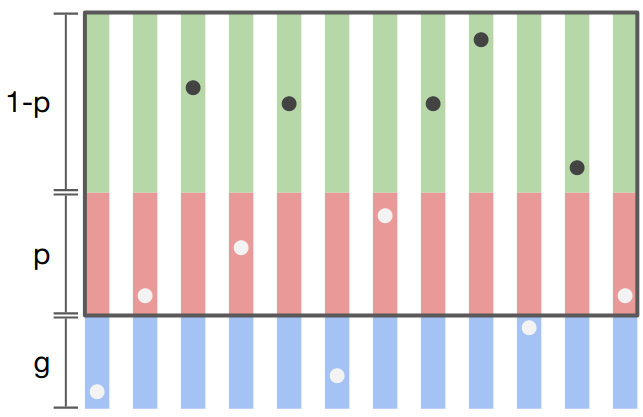
\includegraphics[height=4cm, clip]{figures/chernoff}
            \caption{{
                We sample points uniformly at random on $N$
                sticks, each with three parts: \textbf{green}
                with length $1-p$, \textbf{red} with length $p$, and
                \textbf{blue} with length $g$.  We call non-blue points
                \textbf{boxed} and non-green points \textbf{hollow}.
            }}
            \label{fig:chernoff}
        \end{figure}
        \begin{proof} \renewcommand{\qedsymbol}{}
            Let our coin flips arise from sampling points on sticks
            (Figure \ref{fig:chernoff}), where green means tails, red
            means heads, and we condition on the event that blues do not occur.
            %
            To show that less than $(p+g)N = p^\prime N$ flips are
            heads is to show --- given that all points are \textbf{boxed} ---
            that less than $p^\prime N$ points are red. 
            %
            For any $M$:
            {%
            \begin{align*}
                    & ~ \Pp[\text{$M$ are red $\mid$ all are boxed}] \\
                  = & ~ \frac{\Pp[\text{all hollows are red $\mid$ $M$ hollow}] \cdot \Pp[\text{$M$ are hollow}]}{\Pp[\text{all are boxed}] } \\
                  = & ~ (1 - g/p^\prime)^{M} \cdot (1+g)^{N} \cdot \Pp[\text{$M$ are hollow}]
            \end{align*}
            }%
            We sum over $M\geq p^\prime N$, bound $\Pp[\cdots p^\prime N \cdots] \leq 1$,
            then invoke $(x \mapsto x^{p^\prime})$'s concavity and
            $\exp$'s convexity:
            \begin{align*}
                &~\Pp[\text{at least $p^\prime N$ are red $\mid$ all are boxed}]
                \\ \leq
                &~(1 - g/p^\prime)^{p^\prime N} \cdot (1+g)^{N} \cdot \Pp[\text{at least $p^\prime N$ are hollow}]
                \\ \leq
                &~(1 - g)^N \cdot (1 + g)^{N}
                =
                (1 - g^2)^N
                \leq
                \exp(- Ng^2)
                ~~~~~\square
            \end{align*}
        \end{proof}
        The Chernoff bound gives us the control over tails we would expect from the
        Central Limit Theorem, but for finite instead of asymptotically large
        $N$.  In particular, when we learn from much but finite data, the
        training error will \textbf{concentrate} near the testing error.

        Indeed, for any $f\in \Hh$, $\Ein(f)$ is the average of $N$ independent 
        Bernoullis of mean $\Eout(f)$.  So for finite $\Hh$, the gap is
        probably small:
        \begin{align*}
            &~\Pp_{\Ss\sim \Dd^N}[\Egap(\Ll) \geq g] \\
            \leq 
            &~\sum_{f\in \Hh} \Pp_{\Ss\sim \Dd^N}[\Eout(f) \geq \Ein(f) + g] \\
            \leq
            &~|\Hh| \cdot \exp(-Ng^2)
        \end{align*}

        For example, if $\Hh$ is parameterized by $P$ numbers, each represented
        on a computer by $32$ bits, then $|\Hh|\leq 2^{32 P}$ and, with
        probability $1-\delta$, the gap is less than
        $$
            \sqrt{(\log(1/\delta) + 32 P)/N}
        $$
        This bound's sensitivity to the description length $32 P$ may seem
        artificial.  Indeed, the various $\Hh$ used in practice --- e.g.\
        linear models or neural networks --- depend smoothly on their
        parameters, so the parameters' least significant bits barely affect 
        the classifier.  In other words, $\Hh$'s cardinality is not an apt
        measure of its size.  The VC-dimension measures $\Hh$ more subtly.

      \samsubsubsection{quadratic forms}
      \samsubsubsection{covariance, correlation, least squares regression}

    \samsubsection{bayesian inference}
      \samquote{
        So little of what could happen does happen.
      }{salvador dal\'i}

      \samsubsubsection{conceptual framework}
      We're confronted with an observation or dataset $\sfo$ that comes from
      some unknown underlying pattern $\sfh$.  We know how each possible value
      $h$ for $\sfh$ induces a distribution on $\sfo$ and we have a prior sense
      of which $h$s are probable.  Bayes' law helps us update this sense to
      account for the dataset by relating two functions of $h$:
      $$
        \underbrace{p_{\sfh|\sfo}(h|o)}_{\text{posterior}}
        \propto
        \underbrace{p_{\sfo|\sfh}(o|h)}_{\text{likelihood}}
        \cdot
        \underbrace{p_{\sfh}(h)}_{\text{prior}}
      $$

      Bayes' law underlies most of our analyses throughout these
      notes.\marginnote{%
        $\leftarrow$ Like Newton's $F=ma$, Bayes is by itself inert: to make predictions
        we'd have to specify our situation's forces or likelihoods.  Continuing
        the metaphor, we will rarely solve our equations exactly; we'll instead
        make approximations good enough to build bridges and swingsets.  Still,
        no one denies that $F=ma$ orients us usefully in the world of physics.
        So it is with the law of Bayes.
      }

      Formally, we posit a set $\hH$ of \emph{hypotheses}, a set $\oO$ of
      possible \emph{observations}, and a set $\aA$ of permitted
      \emph{actions}.  We assume as given a joint probability measure
      $p_{\sfo,\sfh}$ on $\oO\times \hH$ and a \emph{cost function}
      $c:\aA\times \hH \to \Rr$.
      %
      That cost function says how much it hurts to take the action $a\in \aA$
      when the truth is $h\in \hH$.
      %
      Our primary aim is to construct a map $\pi:\oO\to \aA$ that makes the
      expected cost $\Ee_{\sfh,\sfo} \, c(\pi(\sfa); \sfh)$ small.

      Below are three examples.  In each case, we're designing a robotic vacuum
      cleaner: $\hH$ contains possible floor plans; $\oO$, 
      possible readings from the robot's sensors.  The examples differ in how
      they define and interpret $\aA$ and $c$.

      \textbf{A}.  $\aA$ consists of probability distributions over $\hH$. We
      regard $\pi(o)$ as giving a posterior distribution on $\hH$ upon
      observation $o$.  Our cost $c(a;h)$ measures the surprise of someone who
      believes $a$ upon learning that $h$ is true. 
      %
      Such \emph{inference problems}, being in a precise sense universal, pose
      huge computational difficulties; we thus often collapse distributions to
      points, giving rise to the distinctive challenge of balancing estimation
      error with structural error.

      \textbf{B}.
      $\aA$ consists of latitude-longitude pairs, interpreted as a guessed
      location of the robot's charging station.  The cost $c(a;h)$ measures how
      distant our guess is from the truth.  
      %
      Such \emph{estimation problems} abound in science and engineering; they
      pose the distinctive challenge of balancing
      sensitivity-to-misleading-outliers against
      sensitivity-to-informative-datapoints.
      %robustness to measurement noise with
      %centeredness. 

      \textbf{C}.  $\aA$ consists of instructions we may send to the motors,
      instructions that induce motion through our partially-known room.  The
      cost $c(a;h)$ incentivizes motion into dusty spaces and penalizes bumping
      into walls.
      %
      We often compose such \emph{decision problems} sequentially; this gives
      rise to the distinctive challenge of balancing exploration with
      exploitation.

      \samsubsubsection{effect of prior choice}
      \samsubsubsection{mixture priors and hierarchy}

      \samsubsubsection{frequentism and choice of prior}
      %\samsubsubsection{uniform priors} % jeffries
        Our engineering culture prizes not just \emph{utility} but also
        \emph{confidence}, since strong guarantees on our designs allow 
        composition of our work into larger systems: equality, unlike
        similarity, is transitive.  For example, we'd often prefer a 99\%
        guarantee of adequate performance over a 90\% guarantee of ideal
        performance.  This asymmetry explains our pessimistic obsession with
        worst-case bounds over best-case bounds, cost functions over fitness
        functions, and simple models with moderate-but-estimatable errors over
        rich models with unknownable-but-often-small errors.

        The \emph{frequentist} or \emph{distribution-free} style of statistics
        continues this risk-averse tradition.  In the fullest instance of this
        style, we do inference as if the true unknown prior on $\hH$ is chosen
        adversarially.
        %
        That is, we try to find $\pi$ that makes the following error small:
        $$
          \max_{p_{\sfh}}
          \,
          \Ee_{\sfh \sim p_{\sfh}(\cdot)} \Ee_{\sfo \sim p_{\sfo}(\cdot|\sfh)}
          \,
          c(\pi(\sfo); \sfh) 
        $$
        %
        %For example, suppose $\aA=\hH$ and $c(a;h) = [\![a\neq h]\!]$ is the
        %zero-one cost.
        %The prior in the minimax pair $(\pi, p_{\sfh})$ tends to be pretty
        %uniform. 
        Intuitively, 

        %minimax 
        %``uniform'' prior
        %on hypothesis space.

      \samsubsubsection{p-hacking} % likelihoods, confidence intervals 
      \samsubsubsection{hidden assumptions} % distribution-existence as coherence condition

      \samsubsubsection{(multiple) hypothesis testing}
      %\samquote{
      %  The theory of probabilities is at bottom nothing but common sense
      %  reduced to calculus; it enables us to appreciate with exactness
      %  [what we] feel with a sort of instinct ...
      %}{pierre simon laplace}

      Let's now consider the case where $\hH$ is a small and finite.  We

  \newpage
  \marginnote[-0.05cm]{%
    \textsc{Table of Contents}
    \begin{description}
      %\item[] \vphantom{.} 
      %  \begin{description}
      %  \end{description}
      \item[A. Prologue] \phdot 
        %\begin{description}
        %  \item[bird's eye framework] \phdot
        %\end{description}
      \item[B. Linear classification] \phdot
        \begin{description}
          \item[linear approximations] \phdot % hypothesis class; briefly mention regression
          \item[iterative optimization] \phdot % perceptron, logistic
          \item[generalization bounds] \phdot % generalization bounds
          \item[model selection] \phdot % validation, featurization from domain knowledge, which objective func?
          \item[priors and generalization] \phdot % priors and regularization
          \item[optimization tricks] \phdot % convex optimization; implicit regularization
          \item[kernels enrich approximations] \phdot
        \end{description}
      \item[C. Nonlinearities] \phdot
        \begin{description}
          \item[fixed featurization] \phdot % classic nonlinearities: discrete-continuous (softmax; embedding); normalization; binning 
          \item[learned featurizations] \phdot
          \item[differentiation] \phdot % smoothness assumption, backprop as dynaprog, autodiff
          \item[architecture and symmetry] \phdot % CNNs, RNNs
          \item[feature hierarchies] \phdot % 
          \item[stochastic gradient descent] \phdot % learning rates as riemannian metrics; conditioning; annealing
          \item[loss landscape shape] \phdot % thinking about minima etc
        \end{description}
      \item[D. Structured inference] \phdot
        \begin{description}
          \item[graphical generative models] \phdot % directed models
          \item[inferring conditional marginals] \phdot
          \item[learning parameters] \phdot % spectre of marginal likelihood; EM, other variational methods, MCMC
          \item[hierarchy and mixtures] \phdot
          \item[hierarchy and transfer] \phdot
          \item[variational and sampling methods] \phdot % - tie in with deep learning 
          \item[amortized inference] \phdot % - tie in with deep learning 
        \end{description}
      \item[E. Reductions to supervision] \phdot
        \begin{description}
          \item[to build a tool, use it] \phdot
          \item[distributions as maps] \phdot
          \item[self-supervised: downstream tasks] \phdot
          \item[self-supervised: autoregression] \phdot
          \item[reinforcement: exploration-exploitation] \phdot
          \item[reinforcement: states and $q$-values] \phdot
              % another paradigm: learning-from-instruction
          \item[beyond i.i.d.] \phdot
        \end{description}
      \item[F. Three brief example projects]   \phdot 
        \begin{description}
          \item[example: flooding plains] \phdot
          \item[example: ancient tablets] \phdot
          \item[example: pairing flavors] \phdot
        \end{description}
      \item[G. Appendices] \phdot 
        \begin{description}
          \item[python refresher] \phdot
          \item[probability refresher] \phdot
          \item[linear algebra refresher] \phdot
          \item[calculus refresher] \phdot
          \item[notes on high dimensions] \phdot
          \item[notes on bayes' law] \phdot
              %
        \end{description}
    \end{description}
  }



\end{document}

